\chapter{Fourier transforms over finite fields and rings}
\label{chap-extension-finite-field-values}
\chapteroverview{Fourier identities also work with exact arithmetic in finite
fields and suitable rings. They lead to integer multiplication without
rounding and to algebraic constructions of error-correcting codes. This
chapter develops the required roots of unity, derives BCH encoding and
decoding, and uses complex-valued Fourier duality to study code parameters.}

\section{Calculations over finite fields}
\label{sect1-calculations-finite-field}
A finite field can play two different roles in Fourier analysis. Earlier
chapters used it as the domain of a complex-valued function. Here the
\emph{values} of the function lie in a finite field as well. The convolution
and inversion identities survive when enough roots of unity are available,
but statements about complex magnitudes or positive inner products do not
carry over automatically.

\subsection{Finite-field Fourier transform}
\label{sect2-trans-fourier-finite-field}
\begin{defn}[Primitive root of unity]
\index{Root of unity!primitive}
An element $\zeta$ of a field $K$ is a primitive $n$th root of unity if
it has multiplicative order exactly $n$: $\zeta^n=1$ and
$\zeta^j\ne1$ for $1\leq j<n$.
\end{defn}
The multiplicative group of $\FF_q$, where $q=p^r$, is cyclic of order
$q-1$. It contains a primitive $n$th root if and only if $n\mid q-1$.
If $\omega$ generates $\FF_q^*$, then $\omega^{(q-1)/n}$ is such a root.
In particular, the characteristic $p$ cannot divide $n$.

\begin{defn}[Finite-field Fourier transform]
Fix a primitive $n$th root $\zeta\in K=\FF_q$. For $f\in K^n$, define
\begin{equation}
\label{eq-defn-transforme-fp}
 \Ff(f)[j]=\wh f[j]=\sum_{k=0}^{n-1}f[k]\zeta^{-kj},\qquad 0\leq j<n.
\end{equation}
\end{defn}
\begin{prop}[Convolution and inversion]
\label{prop-prtes-tfd-finite-field}
The transform is an algebra isomorphism from $K^n$ with unnormalized
circular convolution to $K^n$ with componentwise multiplication. Its
inverse is
\begin{equation}
\label{eq-defn-tfd-finite-field}
 \Ff^{-1}(g)[j]=n^{-1}\sum_{k=0}^{n-1}g[k]\zeta^{kj}.
\end{equation}
Here $n^{-1}$ denotes the inverse of $n\,1_K$, which is nonzero because
$p\nmid n$.
\end{prop}
\begin{proof}
The geometric sum $\sum_{k=0}^{n-1}\zeta^{ks}$ equals $n$ if $n\mid s$
and zero otherwise: in the latter case $1-\zeta^s$ is invertible.
Expanding the two transforms proves inversion. Reindexing the finite sums
in a convolution proves the product rule.
\end{proof}
These calculations are exact. For integer multiplication, the remaining
issue is to choose moduli large enough to recover integer coefficients
from their residues. This replaces the rounding analysis required by a
complex FFT; it does not give a continuous-frequency interpretation to
field-valued coefficients.

\subsection{Choosing a root in the base field}
\label{sect2-a-particular-case}
For $n=p-1$, any generator of $\FF_p^*$ suffices. More generally, if
$n\mid p-1$, raise such a generator to $(p-1)/n$. A candidate $g$ generates
$\FF_p^*$ precisely when
\[
 g^{(p-1)/\ell}\ne1\pmod p
 \quad\text{for every prime divisor $\ell$ of $p-1$}.
\]
This reduces the order check to the prime factors of $p-1$.
See Cohen~\cite{cohen-computational} for computational methods.
If $n\nmid p-1$, an extension field is needed; if $p\mid n$, no finite
extension can supply a primitive $n$th root.

\subsection{Cyclotomic extensions}
\label{sect2-cyclotomic-field}
\begin{thmdefn}[Cyclotomic polynomials]
\label{notation-64}\index{Cyclotomic polynomial}
For $n\geq1$, the cyclotomic polynomial is
\[
 \Phi_n(X)=\prod_{\substack{1\leq k\leq n\\\gcd(k,n)=1}}
                 (X-e^{2\pi\imath k/n}).
\]
It has integer coefficients, is irreducible over $\QQ$, and satisfies
\begin{equation}
\label{eq-decomposition-xn-1}
 X^n-1=\prod_{d\mid n}\Phi_d(X).
\end{equation}
\end{thmdefn}
See Demazure~\cite{demazure} for a proof. The product formula gives a
recursive construction, beginning with
\[
 \Phi_1=X-1,\quad \Phi_2=X+1,\quad
 \Phi_3=X^2+X+1,\quad \Phi_6=X^2-X+1.
\]
Program~\ref{listing-calculus-cyclotomic-polynomials} computes these
polynomials exactly in Python. The case $n=105$ is the first with a
coefficient of absolute value greater than one.
\begin{listing}[H]
\PythonCode{listing-calculus-cyclotomic-polynomials}
\caption{An exact cyclotomic polynomial.}
\label{listing-calculus-cyclotomic-polynomials}
\end{listing}

\begin{prop}[Cyclotomic factorization over a finite field]
\label{prop-cyclotomy-fp}
Assume $n>1$ and $\gcd(n,p)=1$, and let $r$ be the multiplicative order of
$p$ modulo $n$. The reduction of $\Phi_n$ in $\FF_p[X]$ is a product of
distinct irreducible polynomials, all of degree $r$.
\end{prop}
\begin{proof}
The derivative $nX^{n-1}$ is relatively prime to $X^n-1$, so the latter is
square-free. Its cyclotomic factors therefore have disjoint root sets.
A root $\zeta$ of $\Phi_n$ has order $n$: if its order were a proper
divisor $d$, it would also be a root of $X^d-1$, a product of other
cyclotomic factors.

The Frobenius orbit of $\zeta$ is
$\zeta,\zeta^p,\zeta^{p^2},\ldots$. Its length is the least positive $s$
for which $\zeta^{p^s}=\zeta$, namely $r$. The product over this orbit is
fixed by Frobenius, hence has coefficients in $\FF_p$. Every polynomial
over $\FF_p$ vanishing at $\zeta$ vanishes on its entire orbit. Thus the
orbit product is its minimal polynomial and has degree $r$.
\end{proof}
The minimal extension containing a primitive $n$th root is consequently
$\FF_{p^r}$. If $P$ is any irreducible factor of $\Phi_n$ modulo $p$, it can
be realized as
\[
 K=\FF_p[X]/(P),\qquad \zeta=X\bmod P.
\]
The element $\zeta$ generates $K$ as a field over $\FF_p$; it need not
generate the multiplicative group $K^*$. Arithmetic uses polynomials of
degree less than $r$, with coefficients reduced modulo $p$ and products
reduced modulo $P$. In particular, $\FF_{p^r}$ is not $\ZZ/p^r\ZZ$.

\begin{exmp}
Over the integers,
$\Phi_{15}=X^8-X^7+X^5-X^4+X^3-X+1$.
Modulo two it factors as
\[
 \Phi_{15}=(X^4+X+1)(X^4+X^3+1).
\]
The order of $2$ modulo $15$ is $4$. Either factor constructs $\FF_{16}$,
and its indeterminate class has order $15$.
\end{exmp}
The same argument over $\FF_q$ uses the order of $q$ modulo $n$ and the
Frobenius map $x\mapsto x^q$. Integer coefficients are still reduced
modulo the characteristic $p$, not modulo the cardinality $q$.
Factoring over the larger field may split factors that were irreducible
over $\FF_p$.

\begin{rem}
\label{rmk-cyclotomy-cas-special}
If $n=mp^t$ with $p\nmid m$, then
$X^n-1=(X^m-1)^{p^t}$ in characteristic $p$. This describes the repeated
roots, but it does not produce a primitive $n$th root when $t>0$.
The invertible DFT construction in this chapter requires $p\nmid n$.
\end{rem}

\subsection{Transforms in a cyclotomic extension}
\label{sect2-trans-cyclotomic-field}
Once $K$ and $\zeta$ have been constructed, use the same transform formula
for vectors in $K^n$. If the input lies in $\FF_p^n$, its transform may
leave the base field, just as the DFT of a real signal can be complex.
However, inverse transformation recovers the original base-field vector.
The implementation in Section~\ref{sect1-listing-transform-finite-body}
constructs the field, checks the root order, and verifies inversion.

\subsection{Exact convolution and integer products}
\label{sect2-effective-calculations}
Suppose two nonnegative integers are represented by $a$ and $b$ digits
in base $B$. Every coefficient of their linear digit convolution is at most
\[
 \min(a,b)(B-1)^2.
\]
Choose a transform length $n\geq a+b-1$ and pad both digit vectors with
zeros. A prime characteristic $p$ larger than this bound recovers each
coefficient as its unique residue in $\{0,\ldots,p-1\}$. A larger extension
cardinality $p^r$ alone does not increase that integer-recovery range.
Alternatively, use several coprime moduli and reconstruct by the Chinese
remainder theorem; their product must exceed the bound. For signed
coefficients bounded in absolute value by $M$, a modulus greater than
$2M$ permits centered reconstruction.

FFT factorizations remain valid over the field: a subtransform of length
$n/d$ uses the root $\zeta^d$. Radix-two transforms require an odd
characteristic and a power-of-two length. Mixed-radix implementations can
use other factorizations; prime-length leaves can be computed by a direct
sum. Operation counts refer to field operations, whose own cost depends on
the field representation.

\section{Calculations over rings}
\label{sect1-calculations-ring}
A transform over $\ZZ/m\ZZ$ permits exact modular arithmetic without
constructing a field extension. Zero divisors require extra care: merely
choosing a root of the correct order does not guarantee invertibility.
The useful dyadic examples below have odd moduli of the form $2^a+1$.
A nontrivial power-of-two transform cannot be inverted modulo $2^r$,
since its length is not a unit there.

\subsection{Principal roots of unity}
\label{sect2-main-roots}
Throughout, rings are commutative, with $1\ne0$. An element is called
\emph{regular} if multiplication by it is injective; in particular zero
is not regular. This formulation avoids ambiguity in the expression
``not a zero divisor.''
\begin{defn}[Principal root of unity]
\index{Root of unity!principal}
A principal $n$th root in a ring $A$ is an element $\zeta$ such that
$\zeta^n=1$ and every $1-\zeta^j$, $1\leq j<n$, is regular.
\end{defn}
In a field, principal and primitive roots coincide. Over $\ZZ/15\ZZ$,
by contrast, $2$ has order four but is not principal, because
$2^2-1=3$ is a zero divisor.
Some references define principality by vanishing root sums instead.
The regularity condition used here implies those sums and also gives the
injectivity statement below.

\begin{defn}[Fourier maps over a ring]
For a principal $n$th root $\zeta\in A$, set
\begin{equation}
\label{eq-defn-transform-ring}
 \Ff(f)[j]=\sum_{k=0}^{n-1}f[k]\zeta^{-kj},\qquad
 \widetilde\Ff(f)[j]=\sum_{k=0}^{n-1}f[k]\zeta^{kj}.
\end{equation}
\end{defn}
\begin{lem}[Root sums]
\label{lem-transf-fourier-ring}
One has $\sum_{i=0}^{n-1}\zeta^{ki}=n\,1_A$ if $n\mid k$, and zero
otherwise. Moreover, $n\,1_A$ is regular.
\end{lem}
\begin{proof}
Multiplying the sum by $1-\zeta^k$ proves its vanishing when $n\nmid k$.
To prove regularity of $n$, factor
\[
 X^n-1=\prod_{i=0}^{n-1}(X-\zeta^i).
\]
Here is a justification over a ring. After removing the first $j$ monic
linear factors by polynomial division, evaluating at $\zeta^j$ leaves a
product of regular differences times the remaining polynomial value.
Each difference $\zeta^j-\zeta^i$ is a unit times $1-\zeta^{j-i}$,
so the remaining value is zero and the next division is exact.
This induction proves the factorization. Dividing by $X-1$ and evaluating
at $1$ yields
\[
 n\,1_A=\prod_{i=1}^{n-1}(1-\zeta^i).
\]
A product of regular elements is regular.
\end{proof}

\begin{thm}[Fourier transform over a ring]
The map $\Ff$ preserves convolution products and satisfies
$\widetilde\Ff\Ff=\Ff\widetilde\Ff=n\Id$. Both maps are injective.
If $n\,1_A$ is a unit, $\Ff$ is an algebra isomorphism with inverse
$n^{-1}\widetilde\Ff$.
\end{thm}
\begin{proof}
Expanding the composition gives
\[
 (\widetilde\Ff\Ff f)[j]
 =\sum_l f[l]\sum_k\zeta^{k(j-l)}=nf[j].
\]
The other composition is identical with the signs reversed. The root-sum
lemma and regularity of $n$ imply injectivity. Reindexing proves the
convolution identity, and division by $n$ gives the inverse when allowed.
\end{proof}

\begin{prop}[Existence over a residue ring]
\label{prop-cns-existance-ntt}
Let $m=\prod_{i=1}^r p_i^{a_i}$, where the $p_i$ are distinct primes.
A principal $n$th root exists in $\ZZ/m\ZZ$ if and only if
\[
 n\mid\gcd(p_1-1,\ldots,p_r-1).
\]
This condition implies $\gcd(n,m)=1$, so the resulting transform is
invertible.
\end{prop}
Reduction modulo each $p_i$ proves necessity. For sufficiency, lift a
primitive $n$th root from each prime field to $\ZZ/p_i^{a_i}\ZZ$, then
combine the lifts by the Chinese remainder theorem. The lifting argument,
including verification of the $n$th-power identity, is detailed in
Exercise~\ref{exo-demo-cns-existance-ntt}.

\subsection{A dyadic FFT over a ring}
\label{sect2-impl-algo-fft-ring}
\begin{prop}[Principal dyadic roots]
\label{prop-cns-square-root-ring}
For $k\geq1$, an element $\zeta\in A$ is a principal $2^k$th root if and
only if $2\,1_A$ is regular and $\zeta^{2^{k-1}}=-1$.
\end{prop}
Exercise~\ref{exo-root-square-primitive} proves this criterion. It also
shows that $\zeta^2,\zeta^4,\ldots$ provide the roots needed by recursive
half-length transforms.
For $n=2^k$, choose
\[
 m=2^{n/2}+1,\qquad \zeta=2\pmod m.
\]
The modulus is odd and $\zeta^{n/2}=-1$, so the criterion applies whether
or not $m$ is prime. A larger modulus $m=2^{cn/2}+1$ works with
$\zeta=2^c$ for any positive integer $c$; this flexibility is useful when
integer coefficients require a larger recovery range.

\begin{rem}[Fermat numbers]
\label{notation-65}\index{Fermat number}
The Fermat numbers are $\operatorname{Fer}_s=2^{2^s}+1$.
Their first five values are $3,5,17,257,65537$, all prime, whereas
$\operatorname{Fer}_5=4294967297=641\cdot6700417$.
If $2^a+1$ is prime, then $a$ is a power of two: an odd factor greater
than one in $a$ would yield a factorization of $2^a+1$.
Primality is unnecessary for the ring FFT.
\end{rem}
Programs in Section~\ref{sect1-listing-transform-ring} implement this
transform with Python integers, avoiding fixed-width overflow.
Section~\ref{sect1-listing-mult-large-integers-ring} uses it for exact
integer multiplication. The FFT costs $O(n\log n)$ ring operations;
the bit cost of those operations grows with the modulus size.


\section{Error-correcting codes}
\label{sect1-applications-correctors-codes}
\index{Code!error-correcting}
An error-correcting code adds structured redundancy to a message so that
small transmission errors can be detected or corrected. The competing
objectives are a high information rate, reliable recovery, and efficient
encoding and decoding. Finite fields supply useful alphabets and algebraic
constraints; cyclic codes will connect these constraints directly to
Fourier transforms. See~\cite{papini,demazure} for further background.

\subsection{Words, errors, and distance}
We use fixed-length words in $\FF_q^n$. A transmission error changes some
coordinates, giving a received word $y=x+e$. The number of changed symbols,
rather than their magnitudes, measures the error. This model concerns
substitutions in a fixed-length word; insertion and deletion errors require
a different model.

\begin{exmp}[A parity bit]
\label{exmp-bit-parite}
To transmit $a_0,\ldots,a_{n-1}\in\FF_2$, append
$a_n=\sum_{j=0}^{n-1}a_j$. The transmitted word has even parity.
An odd number of bit changes violates this condition and is detected;
an even number is invisible to it. A single parity check does not locate
an error, but appending such a check to another code can increase its
minimum distance.
\end{exmp}

\begin{exmp}[ISBN check digits]
\index{ISBN}
The historical ISBN-10 format uses nine decimal digits followed by a
check symbol $d_9\in\{0,\ldots,10\}$, with $10$ written as X. It satisfies
\[
 \sum_{j=0}^9(10-j)d_j=0\pmod{11}.
\]
The ISBN-10 of the French original is 2-7298-1867-7. A change in a single
symbol produces a nonzero residue. Swapping any two unequal symbols also
produces a nonzero residue, because both the difference of their weights
and the difference of their values are nonzero modulo eleven. These checks
detect such errors but do not, in general, determine their locations.

ISBNs have thirteen digits since 2007~\cite{isbn-agency}. Their check rule
is $d_0+3d_1+d_2+3d_3+\cdots+3d_{11}+d_{12}=0\pmod{10}$.
For example, 9782729818678 identifies the French original. This rule also
detects every single-digit change. Unlike ISBN-10, it can miss an adjacent
swap when the two digits differ by five. The different moduli and weights
lead to different detection properties.
\end{exmp}

\begin{defn}[Hamming weight and distance]
\label{defn-dist-hamming}\label{notation-66}\label{notation-67}
\index{Hamming distance}\index{Hamming weight}
For $x\in\FF_q^n$, let $w(x)$ be its number of nonzero coordinates.
The Hamming distance is $d(x,y)=w(x-y)$, the number of coordinates at
which $x$ and $y$ differ.
\end{defn}
This is a metric: each coordinate where $x$ and $y$ differ must be a
coordinate where $x$ and $z$ differ or where $z$ and $y$ differ, proving
the triangle inequality. On $\FF_2^3$, it is also the shortest-path distance
along the edges of the cube in Figure~\ref{fig-visual-dist-hamming}.
\begin{figure}[tbp]
\centering
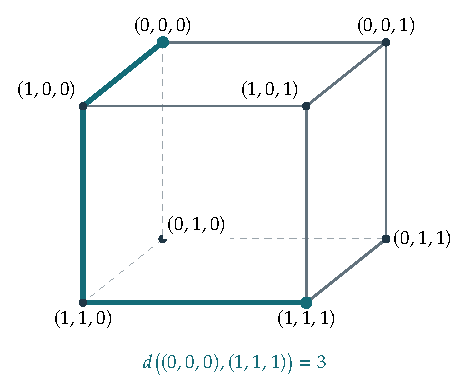
\includegraphics[width=.62\linewidth]{figures/chapter-finite-fields-and-codes/hamming-cube/figure.pdf}
\caption{Hamming distance on $\FF_2^3$. Each cube edge changes one coordinate; the highlighted shortest path has three edges.}
\label{fig-visual-dist-hamming}
\end{figure}

\subsection{Linear codes and their parameters}
\label{sect2-presentation-cyclic-codes}
A code is a nonempty subset $\Cc\subseteq\FF_q^n$. A large code carries
more information, while widely separated codewords permit more errors to
be corrected. Sphere-packing viewpoints help explain this tradeoff;
see~\cite{elkies-ams-1} for connections with discrete geometry.

\begin{defn}[Weight and distance distributions]
\label{notation-68}
For $0\leq i\leq n$, set
\begin{align}
 A_i&=\#\{x\in\Cc:w(x)=i\},\label{eq-defn-weight-distribution}\\
 B_i&=\frac1{|\Cc|}\#\{(x,y)\in\Cc^2:d(x,y)=i\}.
 \label{eq-defn-repartition-distance}
\end{align}
Pairs in the second formula are ordered.
\end{defn}
One has $B_0=1$ and $\sum_iA_i=\sum_iB_i=|\Cc|$.
Translating a code preserves its \emph{distance} distribution, but generally
changes its weight distribution. Translating one of its words to zero is
therefore harmless for distance questions, not for arbitrary weight counts.

For a code with at least two words, define its minimum distance by
$d=\min_{x\ne y\in\Cc}d(x,y)$. It can correct every pattern of at most
$t$ substitutions precisely when its radius-$t$ Hamming balls are disjoint,
which is equivalent to $d\geq2t+1$. Hence its guaranteed correction radius is
$\lfloor(d-1)/2\rfloor$. It can detect every nonzero error of weight at most
$d-1$, although detection alone need not reveal the transmitted word.

\begin{defn}[Linear code]
\index{Code!linear}\index{Generator matrix}
An $[n,m,d]_q$ linear code is an $m$-dimensional subspace of $\FF_q^n$
with minimum distance $d$. A generator matrix $G\in\FF_q^{n\times m}$
has a basis of the code as its columns, so
$\Cc=\{Gu:u\in\FF_q^m\}$ and $|\Cc|=q^m$.
\end{defn}
Changing the basis replaces $G$ by $GU$ for an invertible $m\times m$
matrix $U$ and leaves the code exactly unchanged. Linearity also gives
$A_i=B_i$ and
$d=\min_{0\ne x\in\Cc}w(x)$: for each difference $z\in\Cc$, there are
$|\Cc|$ ordered pairs with $x-y=z$. Linear codes are restrictive, but their
structure makes encoding and many decoding tasks tractable. There is no
general rule that a linear optimum must be much worse than a nonlinear one.

\begin{rem}[Parity-check matrix]
\label{rmk-matrices-control}\index{Parity-check matrix}
A full-row-rank matrix $H\in\FF_q^{(n-m)\times n}$ with $\ker H=\Cc$
is a parity-check matrix. It satisfies $HG=0$, and the syndrome $Hy$
tests membership. Both generator and parity-check matrices are nonunique.
\end{rem}

\begin{exmp}[Repetition]
The binary length-four repetition code has words $0000$ and $1111$, with
\[
 G=\begin{pmatrix}1\\1\\1\\1\end{pmatrix},\qquad
 H=\begin{pmatrix}1&1&0&0\\1&0&1&0\\1&0&0&1\end{pmatrix}.
\]
Its orthogonal code is the even-parity code. Generator and parity-check
matrices exchange roles after transposition; this is explored in
Exercise~\ref{exo-matrices-generator-control}.
\end{exmp}

\begin{exmp}[The cyclic Hamming code of length seven]
\label{exmp-code-hamming-7}
Take the generator matrix, following the column convention,
\[
 G=\begin{pmatrix}
 1&0&0&0\\1&1&0&0\\0&1&1&0\\1&0&1&1\\0&1&0&1\\0&0&1&0\\0&0&0&1
 \end{pmatrix}.
\]
Its columns are successive shifts of the coefficients of $1+X+X^3$.
The sixteen codewords are listed below; the message bits are coordinates
in this chosen basis.
\[
\begin{array}{rrrr}
0000000&1101000&0110100&1011100\\
0011010&1110010&0101110&1000110\\
0001101&1100101&0111001&1010001\\
0010111&1111111&0100011&1001011
\end{array}

\]
The nonzero weights are $3,4,7$, with multiplicities $7,7,1$.
Thus the code has parameters $[7,4,3]_2$ and corrects one error.
It is cyclic because
$(1+X+X^3)(1+X+X^2+X^4)=X^7+1$ in $\FF_2[X]$; the next section
explains why this divisibility guarantees closure under all circular shifts.
\end{exmp}

\begin{prop}[Singleton bound]
\label{prop-borne-singleton}
A linear code with $m\geq1$ satisfies
\begin{equation}
\label{eq-borne-singleton}
 d\leq n-m+1.
\end{equation}
\end{prop}
\begin{proof}
The subspace $E$ whose last $m-1$ coordinates vanish has dimension
$n-m+1$. Since $\dim E+\dim\Cc=n+1$, their intersection contains a
nonzero word. That word has weight at most $n-m+1$.
\end{proof}
Equality defines a \emph{maximum distance separable} (MDS) code.
The bound also has a nonlinear form: puncturing $d-1$ coordinates is
injective on any code of minimum distance $d$, so $|\Cc|\leq q^{n-d+1}$.

\subsection{Cyclic codes}
\label{sect2-cyclic-codes}
Identify $x=(x_0,\ldots,x_{n-1})$ with
$x(X)=\sum_{j=0}^{n-1}x_jX^j$ in $R=\FF_q[X]/(X^n-1)$.
Multiplication by $X$ sends the word to $(x_{n-1},x_0,\ldots,x_{n-2})$.
A linear code is \emph{cyclic} if it is closed under this shift.
It is then an ideal of $R$, because closure under $X$ and linear
combinations implies closure under multiplication by every polynomial.
The converse is immediate.

Every such ideal has a unique monic generator $g$ dividing $X^n-1$.
Indeed, its inverse image in $\FF_q[X]$ is a principal ideal containing
$X^n-1$. The code consists of the ordinary products $ag$ with
$\deg a<n-\deg g$, giving dimension $n-\deg g$. The polynomials
$g,Xg,\ldots,X^{n-\deg g-1}g$ provide generator columns.
This also includes the zero code, with $g=X^n-1$, and the whole space,
with $g=1$.

\subsection{Constructing BCH codes}
\label{sect2-codes-BCH}\index{BCH code}
Fix a prime $p$, a length $n$ coprime to $p$, and a primitive $n$th root
$\alpha$ in a finite extension $K$ of $\FF_p$. For a set
$I\subseteq\ZZ/n\ZZ$, consider
\begin{equation}
\label{eq-defn-pol-gen-codes-bch}
 g_I(X)=\prod_{i\in I}(X-\alpha^i).
\end{equation}
This is a divisor of $X^n-1$ in $K[X]$. To define a code over the base
field, its coefficients must belong to $\FF_p$.

\begin{lem}[Frobenius criterion]
A polynomial $Q\in K[X]$ belongs to $\FF_p[X]$ if and only if
$Q(X)^p=Q(X^p)$.
\end{lem}
\begin{proof}
An element $a\in K$ belongs to $\FF_p$ precisely when $a^p=a$.
For $Q(X)=\sum_j a_jX^j$, the Frobenius identity gives
\begin{equation}
\label{eq-condition-membership-fp}
 Q(X)^p=\sum_j a_j^p X^{pj},
\end{equation}
which equals $Q(X^p)$ exactly when all the coefficients are fixed.
\end{proof}

\begin{prop}[Admissible sets of roots]
\label{prop-cns-cyclotomic-class}
The polynomial $g_I$ belongs to $\FF_p[X]$ if and only if $I$ is invariant
under multiplication by $p$ modulo $n$.
\end{prop}
\begin{proof}
A polynomial over $\FF_p$ vanishing at $\alpha^i$ also vanishes at
$\alpha^{pi}$. Conversely, if multiplication by $p$ permutes $I$, then
$g_I(X)^p=\prod_{i\in I}(X^p-\alpha^{pi})=g_I(X^p)$, so the criterion applies.
\end{proof}

The orbits of this permutation are the $p$-cyclotomic cosets
\begin{equation}
\label{eq-defn-pol-cyclotomic-classes}
 I_k=\{k,pk,\ldots,p^{s-1}k\}\pmod n,
\end{equation}
where $s$ is the least positive integer with $p^sk\equiv k\pmod n$.
They partition all residues, including $I_0=\{0\}$. The polynomial
\begin{equation}
\label{defn-pol-classes-cyclo-codes-bch}
 P_k(X)=\prod_{i\in I_k}(X-\alpha^i)
\end{equation}
is the minimal polynomial of $\alpha^k$ over $\FF_p$: its roots form one
Frobenius orbit, so no proper nonempty subset can be the roots of a factor
over $\FF_p$.

\begin{defn}[Narrow-sense BCH code]
For $2\leq\delta\leq n$, take $I$ to be the union of the cyclotomic
cosets meeting $\{1,\ldots,\delta-1\}$. The cyclic code generated by
$g_I=\operatorname{lcm}(P_1,\ldots,P_{\delta-1})$ is the narrow-sense
BCH code of \emph{designed distance} $\delta$.
\end{defn}
A union of cosets need not be a single coset. The designed distance is a
lower bound, not necessarily the exact minimum distance.

\begin{exmp}[Binary codes of length 31]
Fix $K=\FF_2[\alpha]$ with
$\alpha^5+\alpha^4+\alpha^2+\alpha+1=0$. This irreducible polynomial
has degree five, and $\alpha$ has order $31$. The cosets and minimal
polynomials for this particular root are
\[
\begin{array}{c|l|l}
 k&I_k&P_k(X)\\\hline
 0&\{0\}&X+1\\
 1&\{1,2,4,8,16\}&X^5+X^4+X^2+X+1\\
 3&\{3,6,12,24,17\}&X^5+X^3+1\\
 5&\{5,10,20,9,18\}&X^5+X^3+X^2+X+1\\
 11&\{11,22,13,26,21\}&X^5+X^4+X^3+X^2+1\\
 14&\{14,28,25,19,7\}&X^5+X^2+1\\
 15&\{15,30,29,27,23\}&X^5+X^4+X^3+X+1
\end{array}
\]
Their product is $X^{31}-1$. For designed distance five, the required
cosets are $I_1$ and $I_3$, giving
\[
 g=P_1P_3=1+X+X^2+X^3+X^5+X^6+X^8+X^9+X^{10}.
\]
The resulting code has dimension $31-10=21$.
The program in Section~\ref{sect1-listing-decoding-bch} constructs these
polynomials and verifies that their coefficients lie in the base field.
\end{exmp}

A word $x$ belongs to the code exactly when
\begin{equation}
\label{eq-condition-defn-codes-bch}
 x(\alpha^i)=0,\qquad 1\leq i\leq\delta-1.
\end{equation}
In matrix form, these conditions are $Ax=0$, where
$A=(\alpha^{ij})_{1\leq i\leq\delta-1,\,0\leq j<n}$ has size
$(\delta-1)\times n$ over $K$. Expanding its entries in a basis of
$K/\FF_p$ gives base-field parity checks; the expanded rows need not all
be independent. Equivalently, with Fourier root $\zeta=\alpha^{-1}$,
these are the conditions $\wh x[i]=0$ for $1\leq i<\delta$.

\begin{prop}[BCH distance bound]
\label{prop-dist-minimal-code-bch}
Every nonzero word in the BCH code has weight at least $\delta$.
\end{prop}
\begin{proof}
Suppose a nonzero word has $s<\delta$ nonzero coefficients, at distinct
positions $b_1,\ldots,b_s$. Write it as
$x(X)=\sum_{j=1}^s a_jX^{b_j}$ with $a_j\ne0$. The first $s$ vanishing
conditions give
\[
 \sum_{j=1}^s a_j(\alpha^{b_j})^i=0,\qquad 1\leq i\leq s.
\]
The coefficient matrix is a Vandermonde matrix multiplied by a diagonal
matrix with nonzero entries $\alpha^{b_j}$. Its determinant is nonzero
because these elements are distinct. Hence every $a_j$ would vanish,
a contradiction.
\end{proof}
Consecutive vanishing Fourier coefficients are essential to this argument.
A support-size uncertainty bound alone does not yield the BCH distance
bound. For decoding, write $\delta=2t+1$; then all errors of weight at
most $t$ are uniquely correctable. In the binary narrow-sense case, an
even designed distance can be increased to the next odd one without
changing the code, since the extra even exponent is already in the
Frobenius closure of a smaller exponent.

\subsection{Decoding through the Fourier spectrum}
\label{sect2-decodage-bch}
Suppose $y=x+e$ is received, where $x$ is a codeword and
$\nu=w(e)\leq t$. The known syndromes are
\[
 S_j=y(\alpha^j)=e(\alpha^j),\qquad 1\leq j\leq2t.
\]
These are samples of the error's Fourier spectrum, using the positive
phase specified above. If $J$ is the set of error positions, define
\[
 \sigma(Z)=\prod_{i\in J}(1-\alpha^iZ)
          =1+\sigma_1Z+\cdots+\sigma_\nu Z^\nu.
\]
Its degree is the \emph{actual} number $\nu$ of errors, which may be less
than $t$. The error positions are those $i$ for which
$\sigma(\alpha^{-i})=0$.

Extend $S_j=\sum_{i\in J}e_i\alpha^{ij}$ to every integer $j$.
Substituting each root into $\sigma$ proves the recurrence
\[
 S_j+\sigma_1S_{j-1}+\cdots+\sigma_\nu S_{j-\nu}=0.
\]
Indeed, the left-hand side equals
$\sum_{i\in J}e_i\alpha^{ij}\sigma(\alpha^{-i})$.
This direct derivation fixes the direction of all indices.

\paragraph{Determining the number of errors.}
Form the $t\times t$ Hankel matrix
$T_t=(S_{a+b+1})_{0\leq a,b<t}$. If $u_i=\alpha^i$, then
\[
 T_t=V\operatorname{diag}(e_i u_i)_{i\in J}V^{\mathsf T},\qquad
 V=(u_i^a)_{0\leq a<t,\,i\in J}.
\]
The rectangular Vandermonde matrix $V$ has column rank $\nu$, and the
diagonal matrix is invertible. Thus $\operatorname{rank}T_t=\nu$.
This avoids treating a size-$t$ locator system as invertible when fewer
than $t$ errors occur. If $\nu=0$, all errors vanish.

\paragraph{Finding the locator.}
For $\nu>0$, use the recurrence for $j=\nu+1,\ldots,2\nu$:
\[
 \sum_{l=1}^{\nu}S_{j-l}\sigma_l=-S_j.
\]
The coefficient matrix is $T_\nu$ with its columns reversed, so it is
invertible by the same Vandermonde factorization. It is generally dense,
not triangular. Solving it determines the locator uniquely.
This elementary rank-and-solve procedure is sufficient for the examples;
more efficient recurrence algorithms, such as Berlekamp--Massey, avoid
dense elimination for large correction radii.

\paragraph{Completing the spectrum.}
The recurrence now determines $S_{2t+1},\ldots,S_n$ successively from
known values. Periodicity gives $S_0=S_n$. Inverting the Fourier transform
recovers each error value:
\[
 e_i=n^{-1}\sum_{j=0}^{n-1}S_j\alpha^{-ij}.
\]
Subtract $e$ from the received word. The implementation checks that the
reconstructed errors belong to $\FF_p$, that at most $t$ are nonzero,
and that the corrected word satisfies all BCH checks.

An independent recovery method finds the roots $\sigma(\alpha^{-i})=0$
by testing the $n$ positions, then solves the Vandermonde system
$S_j=\sum_{i\in J}e_i\alpha^{ij}$ for $1\leq j\leq\nu$ to recover their
magnitudes. For binary errors these magnitudes are all one, but this is
not true over a general alphabet. Both methods are implemented and compared
in Section~\ref{sect1-listing-decoding-bch}.
The guarantee assumes at most $t$ errors: if more occur, a nearby
codeword accepted by the checks need not be the one originally transmitted.

\section{Error-correcting codes and Fourier duality}
\label{sect1-codes-correctors-duality}
We now return to complex-valued Fourier analysis on the additive group
$G=\FF_2^n$. Orthogonality of characters relates a linear code to its dual;
for nonlinear codes, the same calculation gives positivity constraints on
the distance distribution. These are the starting point of the linear
programming bound. The reference \cite{macwilliams-codes-correcteurs-1}
develops this combinatorial approach in depth.

\subsection{Weight enumerators}
\label{sect2-polynomials-enumerators-weight}
Unless stated otherwise, $\Cc\subset\FF_2^n$ is a linear code of dimension
$m$. The extension to $\FF_q$ uses additive characters and the substitution
$(X,Y)\mapsto(X+(q-1)Y,X-Y)$; see Exercise~\oldref{exo-generalization-mac-williams}.

\begin{defn}[Dual code]
\label{defn-code-dual}\label{notation-69}
\index{Code!dual}\index{Orthogonal!of a code}
The canonical nondegenerate bilinear form is
\begin{equation}
\label{eq-fbs-canonical-f2}
 \dotp{x}{y}=\sum_{i=0}^{n-1}x_i y_i\in\FF_2.
\end{equation}
The dual code is the orthogonal subspace
\[
 \Cc^\bot=\{x\in\FF_2^n:\dotp{x}{y}=0\text{ for every }y\in\Cc\}.
\]
It has dimension $n-m$, and $(\Cc^\bot)^\bot=\Cc$.
\end{defn}
A code and its orthogonal need not be complementary subspaces. A code
is \emph{self-orthogonal} when $\Cc\subset\Cc^\bot$, and \emph{self-dual}
when equality holds. Self-duality implies $n=2m$, but equality of dimensions
alone is insufficient. Exercise~\oldref{exo-codes-autoduaux} connects
self-duality to invariant polynomials.
\index{Code!self-dual}\index{Code!self-orthogonal}

\begin{defn}[Weight enumerator]
\label{defn-polynomial-enumerator-code}
\index{Polynomial!weight enumerator}
With $A_i=\#\{x\in\Cc:w(x)=i\}$, the weight enumerator is
\[
 W_\Cc(X,Y)=\sum_{i=0}^n A_iX^{n-i}Y^i.
\]
It is homogeneous of degree $n$, with $W_\Cc(1,1)=|\Cc|=2^m$.
\end{defn}
\begin{thm}[MacWilliams identity]
\label{thm-id-mac-williams-correctors-codes}
\index{Identity!of MacWilliams}
For a binary linear code,
\[
 W_{\Cc^\bot}(X,Y)=\frac1{|\Cc|}W_\Cc(X+Y,X-Y).
\]
\end{thm}
This is Theorem~\ref{thm-id-mac-williams}, expressed in coding terminology.
Below we prove a version for arbitrary functions that includes this identity.

\subsection{Codes as functions on a group}
\label{sect2-algebre-group-correctors-codes}
The characters of $G$ are $\chi_a(x)=(-1)^{\dotp{a}{x}}$. Our
unnormalized Fourier transform is
\[
 \wh f(a)=\sum_{x\in G}f(x)\chi_a(x).
\]
For any subset $\Cc\subset G$, its indicator $f_\Cc=\sum_{x\in\Cc}\delta_x$
is one on $\Cc$ and zero elsewhere. For a linear code,
\begin{equation}
\label{eq-equivalence-orthogonalite-caractere2}
 a\in\Cc^\bot\quad\Longleftrightarrow\quad
 \chi_a(x)=1\text{ for every }x\in\Cc.
\end{equation}

\begin{prop}[Transform of an indicator]
\label{prop-trans-fourier-indicator-function}
If $\Cc$ is linear, then $\wh f_\Cc=|\Cc|f_{\Cc^\bot}$.
\end{prop}
\begin{proof}
For $a\in\Cc^\bot$, all summands in $\sum_{x\in\Cc}\chi_a(x)$ equal one.
Otherwise, choose $x_0\in\Cc$ with $\chi_a(x_0)=-1$. Translation by $x_0$
permutes $\Cc$, so this sum equals its own negative and is zero.
\end{proof}
For a nonlinear subset, the orthogonal subspace still exists, but it only
records the linear span of the subset. To retain more information, we work
with the Fourier transform of a function instead.

\begin{defn}[Dual function]
For $f\in\CC[G]$ with nonzero total mass
$M_f=\sum_{x\in G}f(x)$, define $f^\bot=\wh f/M_f$.
\end{defn}
Thus $(f_\Cc)^\bot=f_{\Cc^\bot}$ for a linear code. In general, $f^\bot$
need not be an indicator. The normalization uses total mass, not the
average $M_f/|G|$.
For any function, define
\[
 W_f(X,Y)=\sum_{x\in G}f(x)X^{n-w(x)}Y^{w(x)}.
\]
This agrees with the code's enumerator when $f=f_\Cc$.

\begin{thm}[MacWilliams identity for functions]
\label{thm-id-mac-williams-functions}
If $M_f\ne0$, then
\begin{equation}
\label{eq-id-mac-williams-function}
 W_{f^\bot}(X,Y)=\frac1{M_f}W_f(X+Y,X-Y).
\end{equation}
\end{thm}
\begin{proof}
Interchange the two finite sums to obtain
\[
 W_{\wh f}(X,Y)=\sum_{y\in G}f(y)
       \sum_{x\in G}(-1)^{\dotp{x}{y}}X^{n-w(x)}Y^{w(x)}.
\]
The inner sum factors coordinate by coordinate:
\[
 \prod_{j=0}^{n-1}(X+(-1)^{y_j}Y)
       =(X+Y)^{n-w(y)}(X-Y)^{w(y)}.
\]
Division by $M_f$ gives the identity.
\end{proof}

\subsection{Distance distributions of arbitrary codes}
Let $\Cc\subset\FF_2^n$ be nonempty; linearity is no longer assumed.
Its distance function, with the usual unnormalized convolution, is
\begin{equation}
\label{eq-expression-function-distance}
 D_\Cc=\frac1{|\Cc|}f_\Cc*f_\Cc
       =\frac1{|\Cc|}\sum_{x,y\in\Cc}\delta_{x+y}.
\end{equation}
In particular, $D_\Cc(0)=1$, and
\begin{equation}
\label{eq-val-average-dual-function}
 M_{D_\Cc}=|\Cc|.
\end{equation}
If $\Cc$ is linear, each element has exactly $|\Cc|$ decompositions as
$x+y$ with $x,y\in\Cc$, so $D_\Cc=f_\Cc$.

\begin{prop}[Distance distribution]
\label{prop-repartition-distance-dualite}
Writing $W_{D_\Cc}(X,Y)=\sum_{i=0}^n B_iX^{n-i}Y^i$ gives
\[
 B_i=\frac1{|\Cc|}\#\{(x,y)\in\Cc^2:d(x,y)=i\}.
\]
Consequently, $B_0=1$ and $\sum_iB_i=|\Cc|$.
\end{prop}
\begin{proof}
In characteristic two, $x+y=x-y$, hence $w(x+y)=d(x,y)$. Therefore
\begin{equation}
\label{eq-repartition-distance-resulat-intermediaire}
 \sum_{w(z)=i}D_\Cc(z)=\frac1{|\Cc|}
          \sum_{\substack{x,y\in\Cc\\d(x,y)=i}}1.
\end{equation}
\end{proof}
Over $\FF_q$, replace the second indicator in the convolution by
$\widetilde f_\Cc(x)=f_\Cc(-x)$. This counts differences and gives the
same distance interpretation.

Define the \emph{dual distance distribution} by
\begin{equation}
\label{eq-defn-repartition-distance-duale}
 W_{D_\Cc^\bot}(X,Y)=\sum_{i=0}^n B'_iX^{n-i}Y^i
 =\frac1{|\Cc|}W_{D_\Cc}(X+Y,X-Y).
\end{equation}
For a linear code, it is the distance distribution of $\Cc^\bot$.
For a nonlinear code, these coefficients need not count the words of
any code. They nevertheless satisfy a strong positivity constraint.

\begin{prop}[Positivity of the dual distribution]
\label{prop-positivite-repartition-duale}
The numbers $B'_i$ are nonnegative rationals. Moreover,
$B'_0=1$ and $\sum_i B'_i=2^n/|\Cc|$.
\end{prop}
\begin{proof}
The convolution theorem gives
\[
 B'_i=\frac1{|\Cc|^2}\sum_{w(a)=i}|\wh f_\Cc(a)|^2\geq0.
\]
Here $\wh f_\Cc(a)$ is an integer, proving rationality. At $a=0$ it
is $|\Cc|$, so $B'_0=1$. Finally, evaluate
\eqref{eq-defn-repartition-distance-duale} at $(1,1)$ and use $B_0=1$:
\[
 \sum_i B'_i=\frac{W_{D_\Cc}(2,0)}{|\Cc|}=
             \frac{2^n}{|\Cc|}.
\]
No assumption that $0\in\Cc$ is needed.
\end{proof}
Nonnegativity, together with the vanishing of $B_1,\ldots,B_{d-1}$ for
a code of minimum distance $d$, produces the linear programming bound
in Exercise~\oldref{exo-terminal-linear-programming}.

\begin{exmp}[Hadamard codes]
The eight-word code $\Aa_8$ in \eqref{eq-code-hadamard-a8} is a linear
$[7,3,4]$ simplex code. Its distance enumerator is $X^7+7X^3Y^4$.
Applying the substitution above gives
\[
 W_{D_{\Aa_8}^\bot}(X,Y)=X^7+7X^4Y^3+7X^3Y^4+Y^7,
\]
the enumerator of a Hamming code. In particular,
\[
 \begin{array}{c|rrrr}i&0&3&4&7\\\hline B'_i&1&7&7&1\end{array}.
\]
For the twelve-word Hadamard code $\Aa_{12}$ of length eleven, distinct
words are at distance six, so $W_{D_{\Aa_{12}}}=X^{11}+11X^5Y^6$.
The dual polynomial is
\[
 \frac{(X+Y)^{11}+11(X+Y)^5(X-Y)^6}{12}.
\]
Its nonzero coefficients are
\[
 \begin{array}{c|rrrrrrrr}
 i&0&3&4&5&6&7&8&11\\\hline
 B'_i&1&55/3&110/3&88/3&88/3&110/3&55/3&1
 \end{array}.
\]
They sum to $512/3=2^{11}/12$, but some are nonintegral. Thus this
formal dual distribution cannot be the weight distribution of a code.
\end{exmp}

\section{Exercises}
\label{sect1-trans-fourier-val-finite-field-exercises}

\begin{exo}[Cyclotomic coefficients]
\label{exo-calculus-pol-cyclotomic}
Use exact Python arithmetic to find the smallest positive index $n$ such
that $\Phi_n$ has a coefficient of absolute value $a$, for successive
integers $a\geq1$. Verify, for $a=1,\ldots,7$, the values
\[
 1,\quad105,\quad385,\quad1365,\quad1785,\quad2805,\quad3135.
\]
Extend the search to $a=27$ with the explicit limit $20615$.
Explain why it suffices to search odd squarefree
indices after $n=1$. We seek a coefficient of absolute value \emph{exactly}
$a$, not merely a polynomial whose largest coefficient has magnitude
at least $a$.
\end{exo}

\begin{exo}[Existence of principal roots]
\label{exo-demo-cns-existance-ntt}
Prove Proposition~\ref{prop-cns-existance-ntt}. Write
$m=\prod_{i=1}^r p_i^{k_i}$ with distinct primes $p_i$.
\begin{enumerate}
\item Show that a principal $n$th root exists in $\FF_p$ exactly when
$n\mid p-1$.
\item Let $a\in\{1,\ldots,p-1\}$ represent such a root and set
$\zeta_0=a^{p^{r-1}}\pmod {p^r}$. Prove both that $\zeta_0^n=1$
and that $\zeta_0\equiv a\pmod p$.
\item Show that $1-\zeta_0^s$ is a unit modulo $p^r$ for $1\leq s<n$.
\item Use the Chinese remainder theorem to prove the criterion over
$\ZZ/m\ZZ$, including its necessity.
\end{enumerate}
\end{exo}

\begin{exo}[Principal dyadic roots]
\label{exo-root-square-primitive}
Let $A$ be a commutative ring with identity, with the definition of a
principal root used in Proposition~\ref{prop-cns-square-root-ring}.
\begin{enumerate}
\item Prove that $\zeta$ is a principal $(nm)$th root if and only if
$\zeta^m$ is a principal $n$th root and $\zeta^n$ is a principal $m$th root.
No coprimality assumption on $n,m$ is imposed.
\item Show that the only possible principal square root of unity is
$-1$, and that it is principal exactly when multiplication by $2$ is
injective on $A$.
\item Deduce that $\zeta$ is a principal $2^k$th root, $k\geq1$, exactly
when $2$ is regular and $\zeta^{2^{k-1}}=-1$.
\end{enumerate}
\end{exo}

\begin{exo}[Boolean functions and Reed--Muller codes]
\label{exo-boolean-functions}
\index{Boolean!function}\index{Function!bent}\index{Code!of Reed--Muller}
For a Boolean function $\widetilde f:\FF_2^n\to\FF_2$, put
$f=(-1)^{\widetilde f}$ and $\Ww f(a)=\sum_xf(x)(-1)^{\dotp{a}{x}}$.
Define its nonlinearity as the least Hamming distance of its truth table
from the truth table of an affine function $\dotp{a}{x}+b$.
\begin{enumerate}
\item Prove that every Boolean function has a unique multilinear
polynomial representation over $\FF_2$, called its algebraic normal form.
Explain why distance from affine functions measures nonlinearity.
\item Show that
\[
 N(f)=2^{n-1}-\tfrac12\max_{a\in\FF_2^n}|\Ww f(a)|.
\]
The constant coefficient $a=0$ must be included. Describe an FWT algorithm.
\item Use Parseval's identity to prove
$N(f)\leq2^{n-1}-2^{n/2-1}$. Show that equality holds precisely when
$|\Ww f(a)|=2^{n/2}$ for all $a$. Such functions are called \emph{bent};
show that they can exist only for even $n$.
\item For $\widetilde h(u,v)=\widetilde f(u)+\widetilde g(v)$, prove that
$\widetilde h$ is bent if and only if both factors are bent. Check
$\widetilde f(u_1,u_2)=u_1u_2$ and construct examples for every positive
even number of variables.
\item For $n\geq1$, the first-order Reed--Muller code $R(1,n)$ consists
of the truth tables of all affine Boolean functions. Determine its length,
dimension, cardinality, and minimum distance. Give FWT-based encoding and
nearest-word decoding algorithms, including the constant affine functions.
\end{enumerate}
Bent functions were introduced in \cite{rothaus-bent}. For cryptographic
applications and bounds beyond the even-dimensional case, see
\cite{passalic-boolean}.
\end{exo}

\begin{exo}[Learning Boolean functions]
\label{exo-learning-boolean-functions}
Let $f:\FF_2^n\to\{-1,1\}$ and let expectations use the uniform measure.
Its normalized Walsh coefficients are $a_s=\mathbb E[f\chi_s]$. We observe
$f(X_1),\ldots,f(X_m)$ at independent uniform points. The following
exercise illustrates Fourier learning; the more elaborate algorithm in
\cite{kushilevitz-learning-decision-tree} also addresses how to find
important coefficients. Recall Hoeffding's bound for independent
$Z_j\in[-1,1]$ with common mean $a$:
\[
 \Pr\!\left(\left|m^{-1}\sum_j Z_j-a\right|\geq\lambda\right)
 \leq2\exp(-m\lambda^2/2).
\]
Set $\operatorname{sign}(0)=1$.
\begin{enumerate}
\item Compute $\mathbb E[(f-h)^2]$ for $h=a_\beta\chi_\beta$.
\item Prove, for any real-valued $h$, that
$\Pr(f(X)\ne\operatorname{sign}h(X))\leq\mathbb E[(f-h)^2]$.
\item For a fixed index $\beta$, estimate
\begin{equation}
\label{eq-calcul-approach-coef-walsh}
 \widetilde a_\beta=\frac1m\sum_{j=1}^m f(X_j)\chi_\beta(X_j).
\end{equation}
If $m\geq2\lambda^{-2}\log(2/\delta)$, prove that with probability at
least $1-\delta$ over the training sample, the classifier
$\varphi_0=\operatorname{sign}(\widetilde a_\beta\chi_\beta)$ satisfies
\[
 \Pr_X(f(X)\ne\varphi_0(X))\leq1-a_\beta^2+\lambda^2.
\]
Here $X$ is a fresh uniform test point.
\item Suppose $\sum_{w(s)>d}a_s^2\leq\alpha$, where $0\leq d\leq n$.
Let $M=\sum_{j=0}^d\binom nj$ and estimate all coefficients with
$w(s)\leq d$ from the same sample. Show that
\[
 m\geq\frac{2M}{\epsilon}\log\frac{2M}{\delta}
 \quad\Longrightarrow\quad
 \Pr_X\!\left(f(X)\ne\operatorname{sign}
       \sum_{w(s)\leq d}\widetilde a_s\chi_s(X)\right)\leq\alpha+\epsilon
\]
with training-sample probability at least $1-\delta$.
This condition concerns the \emph{Walsh spectrum}; its degree need not
equal the degree of the algebraic normal form in the preceding exercise.
\end{enumerate}
\end{exo}

\begin{exo}[Generator and parity-check matrices]
\label{exo-matrices-generator-control}
Let $\Cc\subset\FF_q^n$ have dimension $m$, with a full-column-rank
generator $G\in\FF_q^{n\times m}$ and a full-row-rank parity-check
matrix $H\in\FF_q^{(n-m)\times n}$.
\begin{enumerate}
\item Give generator and parity-check matrices for $\Cc^\bot$.
\item If $G=\begin{pmatrix}I_m\\A\end{pmatrix}$, find $H$ and explain
how this systematic form simplifies message recovery.
\item Show that a coordinate permutation, followed by a change of
message basis, puts any generator in systematic form. Explain which
operation changes the code and which only changes its parametrization.
\end{enumerate}
\end{exo}

\begin{exo}[Hamming codes]
\label{exo-codes-hamming}
\index{Code!of Hamming}\index{Code!simplex}
Let $k\geq2$, $n=2^k-1$, and let the columns of $H\in\FF_2^{k\times n}$
be the distinct nonzero vectors of $\FF_2^k$. Set $\Cc=\ker H$.
\begin{enumerate}
\item Prove that $\Cc$ has parameters $[2^k-1,2^k-1-k,3]$ and explain
single-error decoding by the syndrome.
\item Construct a cyclic Hamming code as a binary BCH code of designed
distance three, using a primitive element $\alpha\in\FF_{2^k}$.
\item Prove that the radius-one balls about its words partition
$\FF_2^n$: the code is \emph{perfect}. Check that the cyclic code in
Example~\ref{exmp-code-hamming-7} is a Hamming code, with a parity-check
matrix in the matching coordinate order.
\item Show that every nonzero word of $\Cc^\bot$ has weight $2^{k-1}$.
Deduce that this dual is a simplex code.
\item Generalize the construction to $\FF_q$ using one representative
of each one-dimensional subspace of $\FF_q^k$. Determine the length,
dimension, minimum distance, and size of a radius-one ball.
\end{enumerate}
\end{exo}

\begin{exo}[Weight enumerators of Hamming codes]
\label{exo-pol-enumerateur-hamming}
Use the preceding exercise, with $n=2^k-1$ and $k\geq2$.
\begin{enumerate}
\item Enumerate the length-seven code of Example~\ref{exmp-code-hamming-7}.
\item Compute $W_{\Cc^\bot}$ from the constant nonzero weight of the
simplex code.
\item Deduce the formula
\[
 W_\Cc(X,Y)=\frac{(X+Y)^n+n(X+Y)^{(n-1)/2}(X-Y)^{(n+1)/2}}{n+1}.
\]
\item Calculate $A_1,\ldots,A_6$, interpreting coefficients beyond the
length as zero. In particular, show that $A_3=n(n-1)/6$.
\item Prove $A_{n-i}=A_i$ by showing that the all-ones word belongs to
$\Cc$.
\end{enumerate}
\end{exo}

\begin{exo}[Extended Hamming code]
\label{exo-code-hamming-extended}
Append an overall parity bit to the length-seven code in
Example~\ref{exmp-code-hamming-7}. Determine the resulting length-eight
code's parameters, list its words, and compute its weight enumerator.
Prove self-duality by checking orthogonality of a generator's columns;
invariance of the weight enumerator under the MacWilliams substitution
alone does not prove equality of the two codes.
\end{exo}

\begin{exo}[Repetition codes]
\label{exo-code-repetition}
For $n\geq2$, let $\Cc=\{(a,\ldots,a):a\in\FF_q\}$.
\begin{enumerate}
\item Determine its dimension, minimum distance, and weight enumerator.
\item Identify $\Cc^\bot$, compute its parameters and enumerator, and
determine exactly when the repetition code is self-dual.
\end{enumerate}
\end{exo}

\begin{exo}[Hadamard codes]
\label{exo-codes-hadamard}
Let $H_n$, $n\geq4$, be a Hadamard matrix whose first row and column are
all ones. Replace $+1$ by $0$ and $-1$ by $1$, and delete the first column.
Let $\Aa_n$ be the code formed by its $n$ rows, and let $\Bb_n$ be their
union with their bitwise complements.
\begin{enumerate}
\item Identify these codes for the Walsh matrix, $n=2^k$. Are codes
constructed from an arbitrary Hadamard matrix necessarily linear?
\item Compute the lengths, cardinalities, and minimum distances of
$\Aa_n$ and $\Bb_n$, using orthogonality of Hadamard rows.
\end{enumerate}
For reference, two constructions give the following codes:
\begin{equation}
\label{eq-code-hadamard-a8}
\begin{array}{c|c}
 \text{Paley construction}&\text{Walsh construction}\\\hline
 0000000&0000000\\1001011&1010101\\1100101&0110011\\
 1110010&1100110\\0111001&0001111\\1011100&1011010\\
 0101110&0111100\\0010111&1101001
\end{array}.
\end{equation}
\end{exo}

\begin{exo}[MDS codes and Krawtchouk polynomials]
\label{exo-polynomials-mds}
Let $\Cc\subset\FF_2^n$ be linear of dimension $1\leq m\leq n-1$,
with weight distributions $(A_i)$ and $(A'_i)$ for $\Cc$ and $\Cc^\bot$.
Define the binary Krawtchouk polynomials by
\begin{equation}
\label{eq-defn-poly-krawtchouk}
 P_k(x)=\sum_{j=0}^k(-1)^j\binom{x}{j}\binom{n-x}{k-j},
 \qquad 0\leq k\leq n.
\end{equation}
For integer arguments, a binomial coefficient is zero when its lower
index lies outside its usual range.
\begin{enumerate}
\item Compare coefficients in the MacWilliams identity to show
$A'_k=2^{-m}\sum_iA_iP_k(i)$.
\item Prove the moment identities
\[
 \sum_{i=0}^{n-k}\binom{n-i}{k}A_i
   =2^{m-k}\sum_{i=0}^k\binom{n-i}{n-k}A'_i,
   \qquad 0\leq k\leq n.
\]
One route differentiates the inverse MacWilliams identity $k$ times in
$X$ and then sets $X=Y=1$.
\item Assume $\Cc$ is MDS, so its minimum distance is $d=n-m+1$.
Prove that $\Cc^\bot$ is MDS with minimum distance $m+1$, and deduce
\[
 \sum_{i=d}^{n-k}\binom{n-i}{k}A_i
    =\binom nk(2^{m-k}-1),\qquad 0\leq k<m.
\]
\item Explain why these equations determine the entire weight distribution,
and show that $A_d=\binom nd$.
\end{enumerate}
\end{exo}

\begin{exo}[The linear programming bound]
\label{exo-terminal-linear-programming}
Let $R(n,d)$ be the largest cardinality of a binary code of length $n$
and minimum distance at least $d$, with $1\leq d\leq n$.
\begin{enumerate}
\item Prove that the distance distribution of any nonempty code obeys
$\sum_{i=0}^nB_iP_k(i)\geq0$ for $0\leq k\leq n$.
\item Show that $R(n,d)$ is bounded by the following linear program and
prove that its feasible set is bounded. Distance $d$ itself is allowed.
\[
 \begin{split}
 \text{maximize }&\sum_{i=0}^n x_i,\\
 \text{subject to }&x_0=1,\quad x_1=\cdots=x_{d-1}=0,\quad x_d,\ldots,x_n\geq0,\\
 &\sum_{i=0}^n x_iP_k(i)\geq0\quad(0\leq k\leq n).
 \end{split}
\]
\end{enumerate}
\end{exo}
